%%%%%%%%%%%%%%%%%%%%%%%%%%%%%%%%%%%%%%%%%
% Paper 1 --- funder deliverable draft
% Framing: methods paper + demonstration (not a regional case-study
% product). Primary contribution = transferable backtest design,
% contrast, and scoring; secondary = what four Celtic/Irish Sea
% gadoids show under that design.
% Locked identity: one treatment (closed-loop ICES Category 1 advice
% rule vs historical realised F). Constant published ICES F_MSY open
% loop is a no-feedback benchmark only (column in tab:results-current;
% not a co-equal policy). Benchmark series is labelled "open-loop F_MSY"
% (never F_target, which is the HCR control point). Open-loop uses
% published ICES F_MSY = Ftar.
% Scope of this PDF: perfect-information short-cut residual-replay
% backtest (true OM SSB, implErr=0, HCR with perfect knowledge of
% biomass; reference OM bh3). Demonstration stocks: four gadoids
% (Celtic/Irish Sea cod and whiting). Do not advertise a future SAM /
% OEM / full-MP upgrade in this draft.
% Companion: abstract.tex, code-to-run.md, supplementary.tex.
% Existing six-stock draft left intact in paper.tex (do not mix).
% Results tables use provisional numbers from the deterministic
% reference-OM run (paper.tex / 06.0_report.Rmd); figures use existing
% SI and report knits (freeze on re-knit if needed).
%%%%%%%%%%%%%%%%%%%%%%%%%%%%%%%%%%%%%%%%%
%!TEX program = xelatex
\documentclass[11pt,a4paper]{article}

\usepackage[margin=2.5cm]{geometry}
\usepackage{amsmath,amssymb}
\usepackage{booktabs}
\usepackage{graphicx}
\usepackage{setspace}
\usepackage{natbib}
\usepackage{tikz}
\usetikzlibrary{arrows.meta,positioning,calc}
\usepackage{hyperref}
\onehalfspacing
\setlength{\parindent}{0pt}
\setlength{\parskip}{0.5em}

\newcommand{\Fmsy}{F_{\mathrm{MSY}}}
\newcommand{\Blim}{B_{\lim}}
\newcommand{\Btrig}{\mathrm{MSY}_{B_{\mathrm{trigger}}}}
\newcommand{\Bmsy}{B_{\mathrm{MSY}}}
\newcommand{\Ftar}{F_{\mathrm{target}}}

\title{Separating advice-rule performance from implementation and
productivity: a historical closed-loop backtest\thanks{Alternative
(regional) title: A backtest of the ICES Category~1 advice rule for
Celtic and Irish Sea gadoids.}}
\author{}
\date{}

\begin{document}
\maketitle

%------------------------------------------------------------------------------
% Paper 1 abstract (ICES JMS / Fish and Fisheries style).
% Framing: methods paper + demonstration (not a regional case-study product).
% Locked identity: one treatment (closed-loop ICES Category 1 advice
% rule vs historical realised F) + one no-feedback benchmark (constant
% published ICES F_MSY = Ftar). Demonstration: four gadoids
% (Celtic/Irish Sea cod and whiting); OM = reference Beverton--Holt (bh3).
% Scope: perfect-information residual-replay backtest (funder deliverable).
% Do not \input this into paper.tex until that draft is retired;
% paper.tex still carries the six-stock (incl. mackerel) working-paper abstract.
%
% Title (locked; set in skeleton.tex):
%   Separating advice-rule performance from implementation and
%   productivity: a historical closed-loop backtest
% Alternative (regional; carried as \thanks in skeleton.tex):
%   A backtest of the ICES Category 1 advice rule for Celtic and
%   Irish Sea gadoids
%
\begin{abstract}
Realised stock trajectories confound fishing, environmental variability,
and the performance of advice frameworks. Retrospective analysis and
management strategy evaluation (MSE) leave a gap: neither isolates an
advice rule from implementation under the productivity that actually
occurred. We present a historical closed-loop \emph{backtest} that holds
observed productivity fixed in an age-structured operating model,
contrasts perfect closed-loop implementation of a harvest control rule
(HCR), as coded, with historical realised fishing mortality, and scores
outcomes against both operational control points and operating-model (OM)
reference points. A constant open-loop path at the published ICES
$F_{\mathrm{MSY}}$ (equal to $\Ftar$ in the advice rule) is retained
only as a no-feedback benchmark. We demonstrate the design with four ICES
Category~1 gadoids in the Celtic and Irish Seas---Celtic Sea cod, Irish
Sea whiting, Irish Sea cod, and Celtic Sea whiting---under perfect
information (true OM SSB; residual replay; zero implementation error)
with the ICES $\pm20\%$ TAC stability clause above $\Btrig$.
Across the four stocks, three outcome patterns emerge:
following the rule would have rebuilt stocks that were subject to
overfishing (realised $F$ above the target fishing mortality $\Ftar$);
the opposite can occur where realised $F$ already sat below $\Ftar$; and
the two yardsticks---ICES control points such as $\Btrig$ and OM MSY
reference points---can disagree, so that a stock scored as rebuilt
against OM MSY biomass may never clear $\Btrig$ under the rule, with the
size of the gap set by the OM stock--recruitment relationship.
\end{abstract}

\noindent\textit{Keywords:} advice; harvest control rule; backtest; maximum sustainable yield; management strategy evaluation; productivity; gadoids.

%------------------------------------------------------------------------------

%==============================================================================
\section{Introduction}
\label{sec:intro}
%==============================================================================

A main objective of advice for commercially targeted stocks is maximum
sustainable yield (MSY). Increasingly this objective is implemented
through harvest control rules (HCRs) with operational control points: a
target fishing mortality ($\Ftar$), a biomass trigger ($\Btrig$) below
which $F$ is reduced, and a biomass limit ($\Blim$) that the rule is
intended to avoid with high probability. These are control points rather
than biological targets; in the ICES advice rule $\Btrig$ is not $\Bmsy$,
and $\Ftar$ need not coincide with $\Fmsy$. Managers and the public
nonetheless often treat being above $\Btrig$ as having achieved MSY
\citep{winker2026rebuilding}.

Stocks managed under such a rule may still be assessed as overfished, and
this is often attributed to environmental change. A single assessment
history cannot, however, separate three explanations: the HCR was
implemented and failed; the HCR was not followed; or productivity was
unfavourable.

The standard assessment diagnostics do not resolve this. Retrospective
analysis tests the consistency of estimates as data accumulate
\citep{mohn1999} but says nothing about HCR performance. Management
strategy evaluation \citep[MSE;][]{punt2016msebestpractice} tests
candidate rules in closed loop, but against hypothetical futures.
Neither isolates the advice rule from implementation under the
productivity that actually occurred.

We therefore run a historical closed-loop simulation---a
\emph{backtest}---as a counterfactual. An age-structured operating model
(OM) is conditioned on the most recent assessment. Observed productivity
is held fixed by using year-specific biology and replaying the estimated
stock--recruitment residuals. The advice rule is applied year by year, so
that each year's advice responds to the simulated stock, and the
resulting trajectories of fishing mortality, spawning stock biomass
(SSB), and catch are compared with the assessed history. The closed loop
is a perfect-information short-cut: the HCR sees true OM SSB and catch
is taken with zero implementation error. As a no-feedback benchmark,
each stock is also projected at a constant $F$ equal to the published
ICES $F_{\mathrm{MSY}}$ (the same value as $\Ftar$ in the advice rule).

Two questions follow. First, would following the advice rule have
resulted in a different stock status, given the productivity that
occurred? Second, does the answer depend on the yardstick: the ICES
control points ($\Btrig$, $\Ftar$) or the MSY reference points of the OM
($\Bmsy$, $\Fmsy$)?

The approach applies to any stock whose advice is based on an HCR and
for which an OM can be conditioned on an assessment. We demonstrate it
with four ICES Category~1 gadoids in the Celtic and Irish Seas: Celtic
Sea cod, Irish Sea whiting, Irish Sea cod, and Celtic Sea whiting
(Table~\ref{tab:casestudy-status}; Figure~\ref{fig:advice-catch}).
Celtic Sea cod and Irish Sea whiting are subject to overfishing ($F$
above $\Ftar$) and are overfished (SSB below $\Blim$). Irish Sea cod has
had $F$ below $\Ftar$ since 2000, yet SSB has declined and is below
$\Blim$. Celtic Sea whiting was fished above $\Ftar$ over the backtest
window, is below it in the latest assessment year, and remains below
$\Blim$.

%==============================================================================
\section{Materials and methods}
\label{sec:methods}
%==============================================================================

The backtest conditions an age-structured OM on the latest assessment, then reuses historical mass, maturity and selectivity-at-age and projects across the backtest years for the assumed stock--recruitment relationship, replaying the recruitment deviations. This maintains the observed productivity, as the HCR is applied each advice year. The ICES reference points from the Stock Assessment Graphs database
(SAG) are used by the HCR. The OM value of $\Bmsy$ is a performance metric. This is not a conventional MSE of unobserved futures. Stock-specific conditioning, start years, and status summaries for the demonstration are given in Section~\ref{sec:demo-stocks}.

\paragraph{Notation.} $\Ftar$ is the HCR target (ICES Category~1
control point); $\Fmsy$ and $\Bmsy$ are OM MSY reference points and are
not equated with the advice-rule targets. In the open-loop benchmark,
published ICES $F_{\mathrm{MSY}}$ is used as the constant $F$ and equals
$\Ftar$ in the advice rule.

\subsection{Advice framework and diagnostic hierarchy}
\label{sec:diag-hierarchy}

The diagnostic procedures used in stock assessment include retrospective analysis of the consistency of estimates, and hindcast cross-validation of prediction skill of observations \citep{Carvalho2021cookbook}. While MSE tests candidate management strategies, that includes monitoring, assessment, and  management actions, in closed loop against a
simulated OM that represents the stock and fishery \citep{punt2016msebestpractice}. Here we combine the approaches  by backtesting a strategy against management
objectives under historical conditions. We ask whether the advice rule would have met its objectives given the productivity that occurred not whether the rule is robust under climate regimes that have not been observed.

The backtest is a perfect-information short-cut: an age-structured OM is
conditioned on the latest assessment, and observed productivity
(year-specific biology plus stock--recruitment residuals) is replayed
inside that OM. Each advice year the HCR is applied to true OM SSB, and
the resulting catch is taken without implementation error. The simulated
SSB, $F$, and catch are then compared with the realised assessment
trajectories. There is no assessment re-fit inside the loop.

\begin{figure}[htbp]
\centering
% Design schematic for the historical closed-loop backtest
% (OM -- three arms -- score). Self-contained TikZ;
% requires \usepackage{tikz} and \usetikzlibrary{arrows.meta,positioning,calc}.
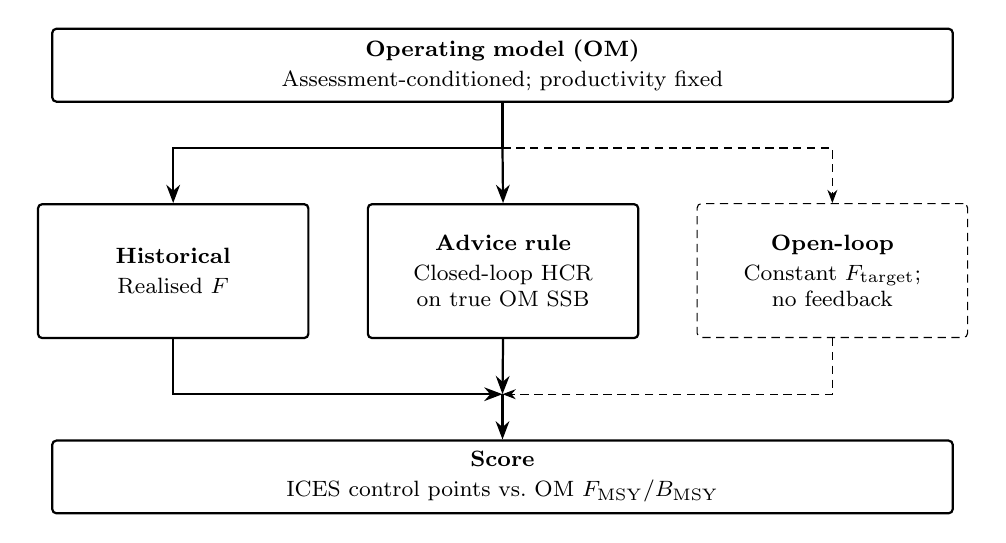
\begin{tikzpicture}[
  font=\footnotesize,
  >=Stealth,
  box/.style={
    draw, thick, rounded corners=1.5pt,
    align=center, inner sep=4pt
  },
  wide/.style={box, text width=0.92\linewidth},
  arm/.style={box, text width=0.26\linewidth, minimum height=1.7cm},
  armdash/.style={arm, densely dashed, thin},
  arr/.style={->, thick}
]
  % Operating model
  \node[wide] (om) {%
    \textbf{Operating model (OM)}\\[0.15em]
    Assessment-conditioned; productivity fixed};

  % Three contrast arms in a matrix (guaranteed equal gap, no overlap)
  \matrix[
    below=1.15cm of om,
    column sep=0.06\linewidth,
    ampersand replacement=\&
  ] (arms) {
    \node[arm] (hist) {%
      \textbf{Historical}\\[0.15em]
      Realised $F$}; \&
    \node[arm] (advice) {%
      \textbf{Advice rule}\\[0.15em]
      Closed-loop HCR\\
      on true OM SSB}; \&
    \node[armdash] (open) {%
      \textbf{Open-loop}\\[0.15em]
      Constant $\Ftar$;\\
      no feedback}; \\
  };

  \coordinate (fork) at ($(om.south)!0.5!(arms.north)$);
  \draw[thick] (om.south) -- (fork);
  \draw[arr] (fork) -| (hist.north);
  \draw[arr] (fork) -- (advice.north);
  \draw[arr, densely dashed, thin] (fork) -| (open.north);

  % Dual scoring
  \node[wide, below=1.15cm of arms] (score) {%
    \textbf{Score}\\[0.15em]
    ICES control points vs.\ OM $\Fmsy$/$\Bmsy$};

  \coordinate (join) at ($(arms.south)!0.5!(score.north)$);
  \draw[arr] (hist.south) |- (join);
  \draw[arr] (advice.south) -- (join);
  \draw[arr, densely dashed, thin] (open.south) |- (join);
  \draw[arr] (join) -- (score.north);

\end{tikzpicture}

\caption{Design of the historical closed-loop backtest. An
assessment-conditioned OM holds productivity fixed. The policy contrast is
\emph{Historical} realised $F$ versus a closed-loop HCR on true OM SSB
(perfect-information short-cut). A subordinate open-loop series holds
published ICES $F_{\mathrm{MSY}}$ ($=\Ftar$ in the advice rule) constant
with no feedback. Outcomes are scored against ICES control points and OM
reference points ($\Fmsy$, $\Bmsy$).}
\label{fig:design}
\end{figure}

\subsection{Operating model}

The OMs are conditioned on the latest ICES assessment for each stock. In the historical window the forward projection retains the assessed time series of weights, natural mortality, maturity, and selectivity. Results reported here use a Beverton--Holt stock--recruitment relationship
\citep{beverton1957dynamics} (hereafter the reference OM) fitted with a
tight prior (CV $=0.001$) on virgin recruitment $R_0$, whose prior value
is set, as coded, from the ratio $\Btrig/\Blim$ of the published ICES
reference points.
% FLAG (dimensional check): 02.0_condition_om.Rmd (bh3) passes
% prior_r0 = MSYBtrigger/Blim (dimensionless, ~1.39) with cv_r0 = 0.001
% to icesdata::eql(model="bevholtSV"). R0 is in recruits, so confirm
% whether eql rescales prior_r0 (e.g. relative to mean recruitment or on
% a log/relative scale) before describing this as a prior "on R0".
% Not resolved from the code; wording above only states what is coded.
HCR control points remain the published ICES values ($\Ftar$, $\Blim$,
and $\Btrig$). The hockey-stick is not re-targeted to OM reference
points, nor is the ICES hockey-stick treated as biological truth; it is
the advice-rule shape and the source of the reference-OM $R_0$ prior
value only.
% Code: OM branch bh3 in eqls; control points on eqls[["bh1"]] (eqs,
% via addBenchmark). Conditioning in Rmd/02.0_condition_om.Rmd.

Multiplicative deviations from the reference-OM stock--recruitment
relationship are replayed with a single iteration: a deterministic
residual history. That fixed productivity is what makes the Historical
versus Advice-rule contrast interpretable.

\subsection{Advice rule}
\label{sec:hcr}

The experiment has one harvest-policy contrast: the closed-loop ICES
Category~1 advice rule versus historical realised $F$. A third
trajectory---open-loop projection at the published ICES
$F_{\mathrm{MSY}}$ (equal to $\Ftar$ in the advice rule) without
biomass feedback, labelled open-loop $\Fmsy$ in figures and tables---is
computed only as a no-feedback reference; that constant is the
advice-rule target, not OM $\Fmsy$. All three share the same OM biology
and residual replay; only the $F$ process differs.

\paragraph{Closed loop}
For each advice year $t$ from 2015 to the stock's terminal year, the
perfect-information short-cut (i)~takes true OM SSB in the last
simulated year as status, (ii)~applies the ICES HCR to set $F$ and thence
catch for $t{+}1$, (iii)~implements that catch on the OM with zero
implementation error, and (iv)~compares SSB, $F$, and catch with the
realised assessment. Status was true OM SSB (perfect knowledge of
biomass; no assessment observation-error model), with residual
deviations from the reference-OM relationship and annual advice. The
advised catch carries the TAC stability clause used in ICES advice under
management strategies: the year-to-year change in TAC is limited to
$\pm20\%$ of the previous catch when SSB is at or above $\Btrig$, and is
unconstrained below the trigger. The clause is tested on the same SSB
that sets $F_{\mathrm{advice}}$.
% Code: err=NULL, implErr=0, interval=1, bndTac=c(0.8,1.2), bndWhen="btrig"
% (R/om.R::hcr_tac_bounds); FLBacktest >= 0.1.7 for the consistent flag.

\paragraph{HCR}
Operational control points follow the generic harvest-control-rule framing
of \citet{winker2026rebuilding}: a target fishing mortality ($\Ftar$), a
biomass trigger below which $F$ is reduced, and a biomass limit ($\Blim$)
that the advice framework is intended to avoid with high probability. In
ICES Category~1 advice the trigger is $\Btrig$ (which maps to
$B_{\mathrm{trigger}}$ in that generic HCR). When biomass is above the
trigger, exploitation proceeds at $\Ftar$; as biomass declines below it,
harvest rates become progressively more restrictive. Control points are
$\Ftar$ (the published ICES $F_{\mathrm{MSY}}$ used as the advice-rule
target), trigger $\Btrig$, $B_{\min}=0$, and
$F_{\min}=0.05\,\Ftar$. The implemented hockey-stick is
\begin{equation}
  F_{\mathrm{advice}}(B)
  \;=\;
  \begin{cases}
  \Ftar
    & \text{if } B \ge \Btrig,\\[0.35em]
  F_{\min}
    + (\Ftar - F_{\min})\,
      \dfrac{B - B_{\min}}{\Btrig - B_{\min}}
    & \text{if } B_{\min} < B < \Btrig,\\[0.75em]
  F_{\min}
    & \text{if } B \le B_{\min},
  \end{cases}
  \label{eq:hcr}
\end{equation}
so the slope runs from $(B_{\min},F_{\min})$ to $(\Btrig,\Ftar)$, not from
$\Blim$ to $\Btrig$: a closure at $\Blim$ is not imposed ($F_{\min}>0$).
Catch advice is a one-year forward projection at $F_{\mathrm{advice}}$.
Published $\Blim$ remains an evaluation threshold for status and scoring,
not the breakpoint of eq.~\eqref{eq:hcr}. The treatment is therefore the
ICES Category~1 MSY rule \emph{as coded} ($F_{\min}=0.05\,\Ftar$, no
closure below $\Blim$). It can differ from advice as issued, which may,
for example, recommend zero catch when SSB is below $\Blim$.
% Code: hcrParams on eqs (SAG on bh1); F_min is the FLBRP-method default.

\paragraph{Benchmark}
\emph{Historical} is the latest WGCSE assessment: realised $F$, catch,
and SSB as assessed, against which the counterfactual is scored.
\emph{Advice rule} is the closed-loop treatment above---the only
``perfect implementation'' claim in this deliverable. The
\emph{open-loop $\Fmsy$} series is a forward projection at constant
published ICES $F_{\mathrm{MSY}}$ (equal to $\Ftar$) from about 1990 to
the terminal year: no SSB feedback and no reduction of $F$ when biomass
is below $\Btrig$. It answers only ``what if fishing had been held at
the published ICES $F_{\mathrm{MSY}}$ with no hockey-stick''. Start years
differ by design: the HCR backtest covers the modern Category~1 MSY rule
from 2015, whereas the open-loop series is a long constant-$F$
reference, not a contemporaneous advice reconstruction. The open-loop
series is therefore a no-feedback reference, and comparing it with the
Advice rule is not a clean isolation of HCR shape: terminal differences
mix rule shape with 25 years of different fishing history before 2015.
The results table (Table~\ref{tab:results-current}) reports Historical,
open-loop $\Fmsy$ (benchmark), and Advice rule; the headline $\Delta$ is
Advice rule minus Historical $\mathrm{SSB}/\Btrig$ only. The published
ICES $F_{\mathrm{MSY}}$ is itself derived from open-loop simulation
(EqSim), so the constant-$F$ projection is its no-feedback analogue
rather than a closed-loop test of the advice rule
\citep{winker2025precautionary}.
% Code: open-loop start = openloop_start (1990, or two years after the
% first assessment year if later).

\subsection{Projection}
Over the historical years, year-specific $M$, mass, and maturity,
together with stock--recruitment residuals, are held common across the
Advice-rule run and the open-loop $\Fmsy$ benchmark. Same productivity
and different $F$ processes are what make the contrast interpretable. We
refer to the period from 2015 to each stock's terminal year as the
\emph{backtest window}; metrics summarising it are labelled
\emph{Current}.

After the terminal year, a 20-year projection (labelled \emph{Future}) is
started from the Historical and Advice-rule terminal states only. No
Future is projected from the open-loop benchmark. The Future uses mean
biology from the equilibrium object, recruitment deviations equal to one
(mean productivity, not a continuation of the residual history), and the
same ICES HCR. It is longer than an ICES one- to two-year advice forecast
and is not a stochastic climate projection.
% Code: Rmd/04.3_rebuild.Rmd.

\subsection{Evaluation}

Two roles for reference points are kept distinct. ICES $\Ftar$, $\Blim$,
and $\Btrig$ are operational control points of the advice rule, held
fixed from SAG. OM $\Bmsy$ and $\Fmsy$ are performance metrics from the
reference OM. Headline Current metrics (Table~\ref{tab:results-current})
are terminal $\mathrm{SSB}/\Btrig$, mean $F$, and mean $F/\Ftar$ over the
backtest window under Historical, the open-loop $\Fmsy$ benchmark, and
the Advice rule, with $\Delta$ equal to Advice-rule minus Historical
$\mathrm{SSB}/\Btrig$. Future metrics (Table~\ref{tab:results-future})
are years from each of the Historical and Advice-rule terminal states to
ICES $\Btrig$ and to OM $\Bmsy$: zero if already above the threshold, and
missing if not reached within twenty years. Probabilities such as
$P(\mathrm{SSB}<\Blim)$, mean yield, and inter-annual catch variability
are standard MSE-style summaries but are not the headline for this
deterministic residual replay.

\paragraph{Software}
Analyses use the FLR packages FLCore, FLBRP, and FLasher
\citep{Kell2007FLR}; the FLBacktest package for the advice rule, the
open-loop and closed-loop projections, and the OM gate
\citep{FLBacktestMethods}; and icesdata for conditioning and SAG
reference points.

\subsection{Demonstration stocks}
\label{sec:demo-stocks}

The demonstration uses four Celtic and Irish Sea gadoids under the ICES
MSY advice basis: Celtic Sea cod (\texttt{cod.27.7e-k}), Irish Sea
whiting (\texttt{whg.27.7a}), Irish Sea cod (\texttt{cod.27.7a}), and
Celtic Sea whiting (\texttt{whg.27.7b-ce-k}). Terminal years of the
cleaned WGCSE assessments used to condition the OMs are 2023 (Irish Sea
cod and whiting), 2024 (Celtic Sea whiting), and 2025 (Celtic Sea cod).
The closed-loop treatment starts in 2015. The open-loop $\Fmsy$ benchmark
starts in 1990, or two years after the first assessment year if later.
The exercise is a counterfactual backtest, not a statutory re-assessment
of advice.
% Inventory: data/reference/stocks.csv.

Initial screening compares ICES advised catch from the Advice and
Scenarios Database (ASD) with reported catch from the latest SAG
assessment year (Figure~\ref{fig:advice-catch}). Years in which reported
catch exceeds advice mark an implementation gap, so depleted terminal
status alone cannot distinguish advice not followed from HCR failure
under the productivity that occurred.

\begin{figure}[htbp]
\centering
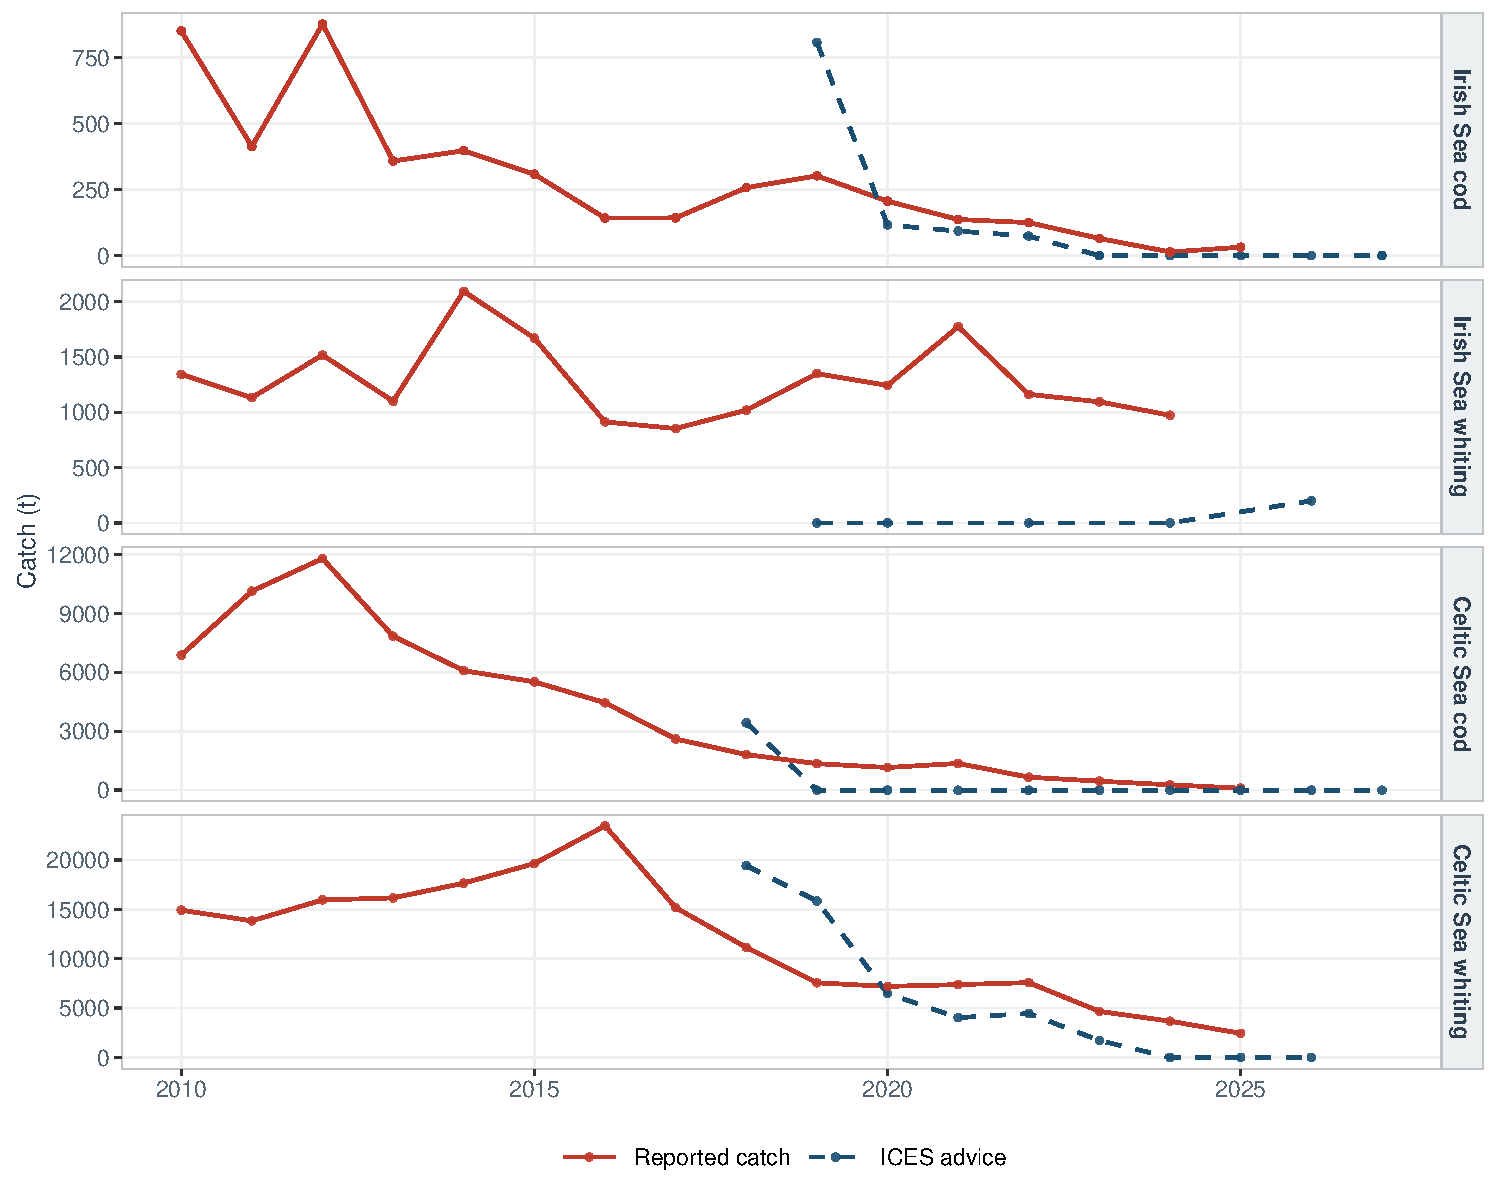
\includegraphics[width=\textwidth]{figs/advice_catch_casestudy.pdf}
\caption{ICES advised catch (ASD) and reported catch (SAG) for the four
demonstration stocks, 2010 onward. Facets use independent $y$-axes
(tonnes).}
\label{fig:advice-catch}
\end{figure}
% Source: Rmd/01_screening.Rmd (S3.2 ICES advice vs reported catch).

SAG screening places all four stocks below $\Blim$ in the latest
assessment year (Table~\ref{tab:casestudy-status}): Celtic Sea cod and
Irish Sea whiting with $F/\Ftar>1$; Irish Sea cod and Celtic Sea whiting
with $F/\Ftar<1$. These are terminal-year values from the latest SAG
assessment; for Celtic Sea whiting the mean over the backtest window was
above $\Ftar$ (Section~\ref{sec:res-scoring}). The terminal-year contrast
frames the Historical versus Advice-rule comparisons below and
anticipates the outcome patterns in Section~\ref{sec:results}.

\begin{table}[htbp]
\centering
\caption{Latest SAG terminal-year status for the four demonstration
stocks. Ratios use published ICES $\Blim$, $\Btrig$, and $\Ftar$.
Values are from the latest SAG assessment (column ``Ass.''), which can be
a later vintage than the WGCSE assessment used to condition the OM (e.g.\
Irish Sea cod: SAG terminal year 2026; conditioning assessment ends
2023). Absolute SSB, $F$, and reference-point values are in the
supplementary status table.}
\label{tab:casestudy-status}
\begin{tabular}{@{}lrrrrr@{}}
\toprule
Stock & Ass. & Year &
  SSB/$\Btrig$ & SSB/$\Blim$ & $F/\Ftar$ \\
\midrule
Celtic Sea cod     & 2026 & 2025 & 0.02 & 0.02 & 4.95 \\
Irish Sea whiting  & 2025 & 2024 & 0.53 & 0.73 & 4.14 \\
Irish Sea cod      & 2026 & 2026 & 0.28 & 0.38 & 0.05 \\
Celtic Sea whiting & 2026 & 2025 & 0.26 & 0.36 & 0.65 \\
\bottomrule
\end{tabular}
\end{table}
% Source: Rmd/01_screening.Rmd (S3.5 Latest stock status).

%==============================================================================
\section{Results}
\label{sec:results}
%==============================================================================

Results are from a single deterministic run of the reference OM under
perfect information. They are reported for two periods: the backtest
window (2015 to each stock's terminal year), which answers whether
following the rule would have changed status; and the 20-year projection
from the terminal year, which answers whether the answer depends on the
yardstick. Figure~\ref{fig:traj} shows the Historical and Advice-rule
trajectories of $F$, SSB, recruitment, and catch for the four stocks
across both periods. The open-loop $\Fmsy$ benchmark is reported in
Table~\ref{tab:results-current} and in the supplementary figures only.
% Figure from scripts/main_traj_facet.R (same series as 06.0_report traj-1..4).

\begin{figure}[htbp]
\centering
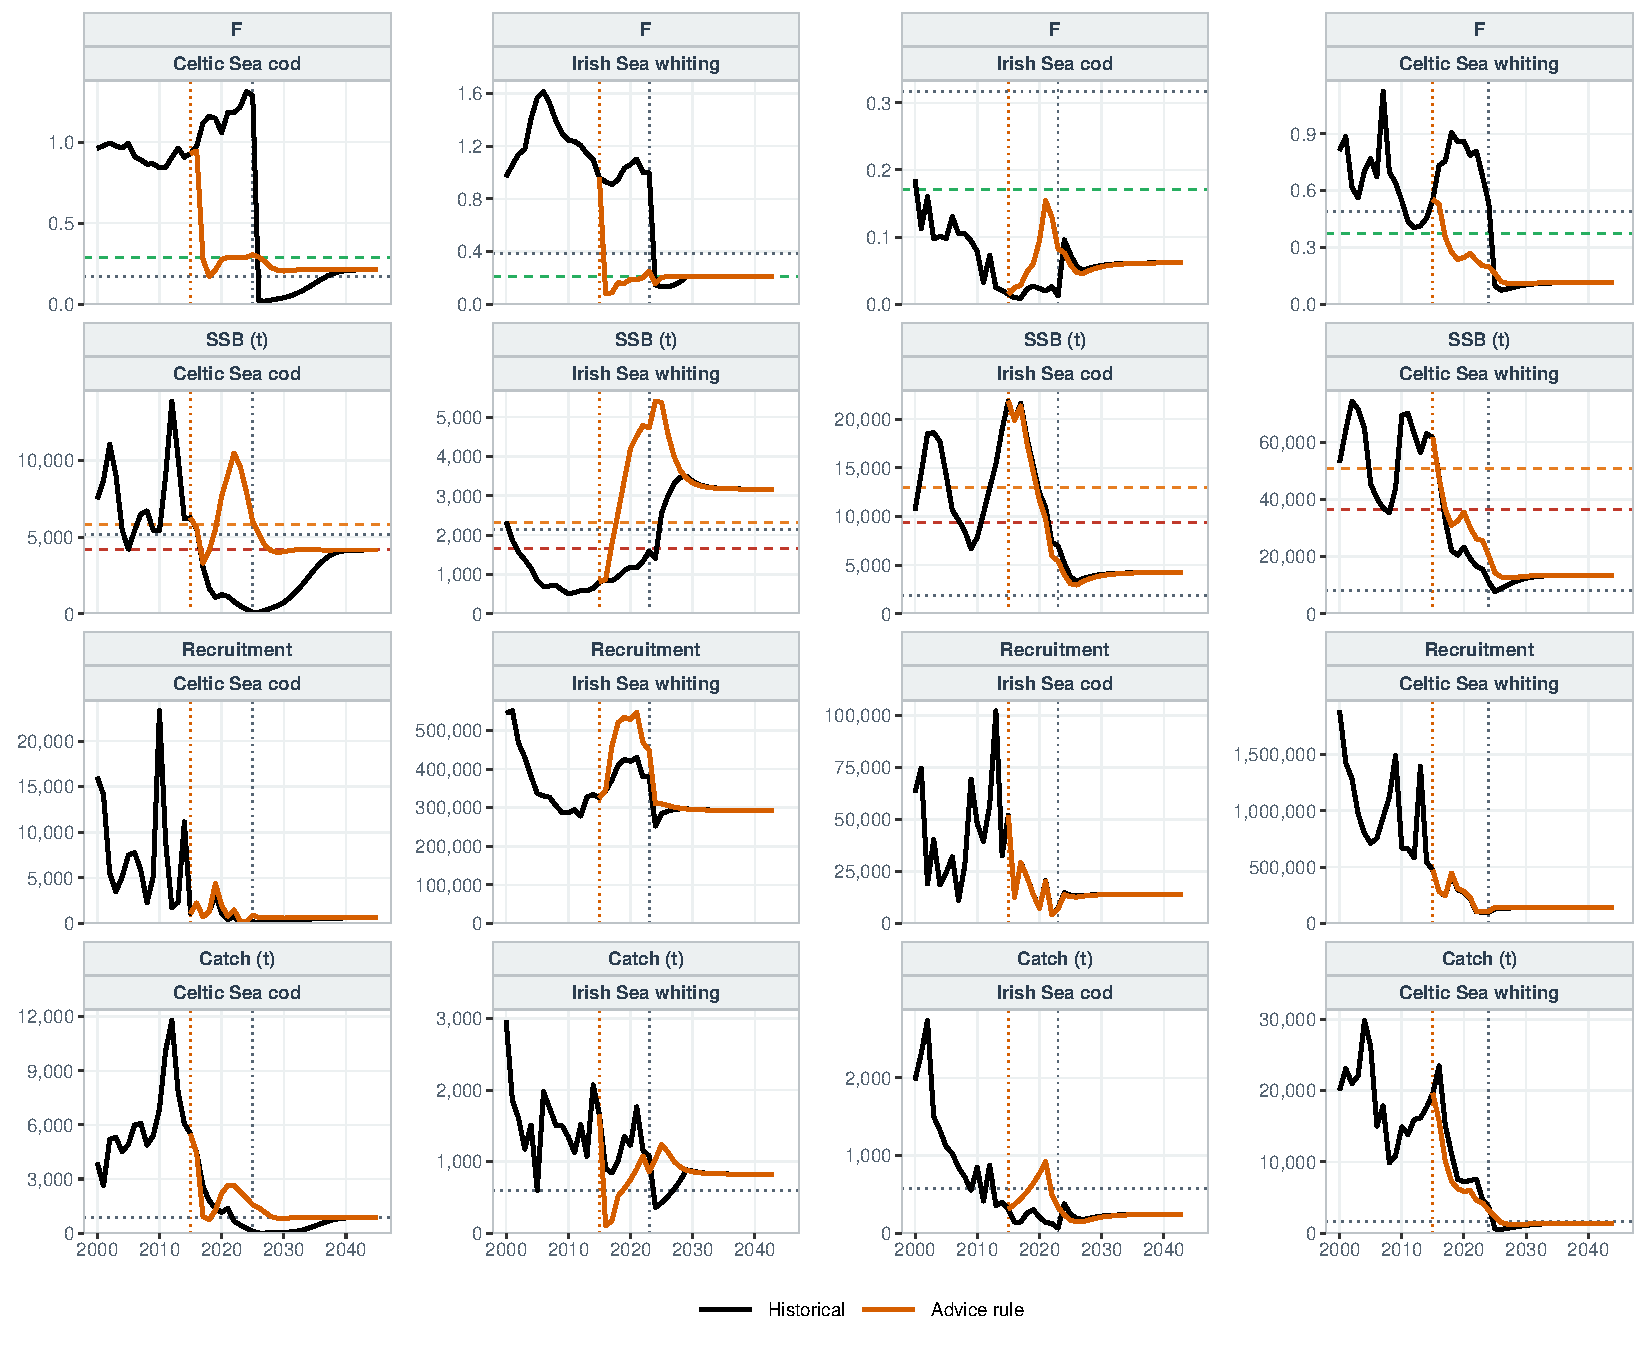
\includegraphics[width=\textwidth]{figs/traj_facet.pdf}
\caption{Historical (black) and Advice-rule (orange) trajectories of
$\bar F$, SSB, recruitment, and catch (rows) for Celtic Sea cod, Irish
Sea whiting, Irish Sea cod, and Celtic Sea whiting (columns). The Advice
rule departs from history in 2015 (orange dotted vertical line); the grey
dotted vertical line marks the terminal year of the conditioning
assessment, after which both series are 20-year HCR projections at mean
recruitment. Dashed horizontal lines are ICES control points: $\Ftar$
(green) on $F$; $\Btrig$ (orange) and $\Blim$ (red) on SSB. Grey dotted
horizontal lines are OM reference points: $\Fmsy$, $\Bmsy$, and MSY.
Panels have independent $y$-axes. Reference OM.}
\label{fig:traj}
\end{figure}

\subsection{Backtest window: would following the rule have changed status?}
\label{sec:res-backtest}

Table~\ref{tab:results-current} summarises the backtest window by
terminal $\mathrm{SSB}/\Btrig$ and by mean $F$ and $F/\Ftar$ over
2015 to the terminal year, for Historical, the open-loop $\Fmsy$
benchmark, and the Advice rule.

For the two stocks subject to overfishing the answer is yes.
Realised $\bar F$ sat well above $\Ftar$ (Celtic Sea cod $F/\Ftar
\approx 3.9$; Irish Sea whiting $\approx 4.7$), and following the rule
would have left terminal SSB at or above $\Btrig$ (cod $\approx 1.0$;
whiting $\approx 2.0$; $\Delta \approx +1.0$ and $+1.4$). Mean
Advice-rule $F/\Ftar$ exceeds 1 (1.34 and 1.20) because the TAC
stability clause holds catch near its historical level while SSB is
still above the trigger in the first year of the rule; once SSB is
below $\Btrig$ the clause no longer applies and $F$ tracks the
hockey-stick. The open-loop $\Fmsy$ path ends at a similar SSB, so the
gain comes from fishing at $\Ftar$ rather than from the hockey-stick
slope; because the two series start 25 years apart this is an
indication, not a decomposition.

For Irish Sea cod the sign reverses. Historical $F/\Ftar \approx 0.11$,
and the rule as coded would have \emph{lowered} terminal
$\mathrm{SSB}/\Btrig$ from $0.54$ to $0.42$ ($\Delta \approx -0.12$),
because the single-stock $F$ implied by $\Ftar$ is higher than realised
$F$. With SSB above $\Btrig$ in 2015, the stability clause limits the
rise in catch to 20\% a year, so $F$ climbs from 0.02 to a peak of 0.15
in 2021 rather than jumping to $\Ftar$ (Figure~\ref{fig:traj}); the
open-loop $\Fmsy$ path, which has no such clause, ends lower still
($0.32$). Catch sat below what the rule would have allowed. Part of
that gap may reflect advice as issued, which can be more restrictive
than the coded rule below $\Blim$; mixed-fishery choke, recovery TACs,
or a mismatch between $\Ftar$ and OM $\Fmsy$ are candidate mechanisms
not identified here.

For Celtic Sea whiting the rule helps but does not rebuild. Mean
$F/\Ftar$ over the window was $2.0$; the Advice rule cuts it to $0.82$
because simulated SSB falls below $\Btrig$ early in the window, so the
hockey-stick keeps $F$ below target. Terminal $\mathrm{SSB}/\Btrig$
rises only from $0.22$ to $0.40$, and the open-loop $\Fmsy$ path also
ends below trigger ($\approx 0.32$). Under this stock--recruitment
relationship and these residuals, neither the rule nor constant $\Ftar$
clears $\Btrig$ by the terminal year.

\subsection{Projection from the terminal year: does the answer depend on the yardstick?}
\label{sec:res-scoring}

Table~\ref{tab:results-future} gives the years from each terminal state
(Historical and Advice rule) to ICES $\Btrig$ and to OM $\Bmsy$ under the
HCR at mean recruitment. On the reference OM, $\Bmsy$ lies below
$\Btrig$ for all four stocks: by about 10\% for Celtic Sea cod and
Irish Sea whiting, and by a factor of six to seven for Irish Sea cod
and Celtic Sea whiting. The two yardsticks therefore disagree in one
direction, and the size of the disagreement is set by the OM
stock--recruitment relationship.
% FLAG: the Bmsy/Btrig ratios for Irish Sea cod and Celtic Sea whiting
% depend on the bh3 R0 prior (Rmd/02.0_condition_om.Rmd); see Methods.

Where the gap is small the yardsticks agree on the outcome. Irish Sea
whiting reaches both thresholds within 2 years from the Historical
state and is already above both from the Advice-rule state. Celtic Sea
cod is above both from the Advice-rule state; from the Historical state
(SSB at 2\% of $\Btrig$) the HCR at mean recruitment reaches neither
within 20 years.

Where the gap is large, a stock scored as rebuilt against OM $\Bmsy$
remains ``below trigger'' indefinitely. Irish Sea cod and Celtic Sea
whiting are already above OM $\Bmsy$ at both terminal states, yet under
the HCR at mean recruitment SSB settles at roughly a third of $\Btrig$
(Figure~\ref{fig:traj}) and never reaches the trigger from either start.
Because the hockey-stick reduces $F$ below the trigger, the HCR
equilibrium on this OM sits between OM $\Bmsy$ and $\Btrig$: the
trigger is not attainable under the rule with this productivity. A
20-year mean-recruitment HCR projection can therefore look like a
successful rebuild against OM $\Bmsy$ while failing on the ICES scale,
and which reading is correct depends on whether the OM
stock--recruitment relationship or the ICES control points better
describe the stock.

\begin{table}[htbp]
\centering
\caption{Backtest window: terminal $SSB/\Btrig$, mean $\bar F$, and mean
$\bar F/\Ftar$ over 2015 to the terminal year for Historical, open-loop
$\Fmsy$ (no-feedback benchmark; published ICES $F_{\mathrm{MSY}}=\Ftar$),
and Advice rule (treatment), plus $\Delta$ (Advice rule $-$ Historical
$SSB/\Btrig$). Deterministic reference-OM run; the Advice rule carries
the $\pm20\%$ TAC stability clause above $\Btrig$.}
\label{tab:results-current}
\resizebox{\textwidth}{!}{%
\begin{tabular}{@{}l rrr rrr rrr r@{}}
\toprule
 & \multicolumn{3}{c}{Historical}
 & \multicolumn{3}{c}{Open-loop $\Fmsy$}
 & \multicolumn{3}{c}{Advice rule}
 & AR $-$ Hist \\
\cmidrule(lr){2-4}\cmidrule(lr){5-7}\cmidrule(lr){8-10}\cmidrule(lr){11-11}
Stock & $SSB/\Btrig$ & $F$ & $F/\Ftar$
      & $SSB/\Btrig$ & $F$ & $F/\Ftar$
      & $SSB/\Btrig$ & $F$ & $F/\Ftar$
      & $\Delta$ \\
\midrule
Celtic Sea cod     & 0.02 & 1.14 & 3.94 & 1.24 & 0.29 & 1 & 1.03 & 0.39 & 1.34 & 1.01 \\
Irish Sea whiting  & 0.68 & 0.99 & 4.73 & 2.01 & 0.21 & 1 & 2.03 & 0.25 & 1.20 & 1.35 \\
Irish Sea cod      & 0.54 & 0.02 & 0.11 & 0.32 & 0.17 & 1 & 0.42 & 0.07 & 0.41 & $-$0.12 \\
Celtic Sea whiting & 0.22 & 0.75 & 1.99 & 0.32 & 0.38 & 1 & 0.40 & 0.31 & 0.82 & 0.18 \\
\bottomrule
\end{tabular}%
}
\end{table}

\begin{table}[htbp]
\centering
\caption{Projection from the terminal year: years to ICES $\Btrig$ and
to OM $\Bmsy$ from the Historical and Advice-rule terminal states under
the HCR (0 = already above; {--} = not reached within 20 years), with the
ratio of OM $\Bmsy$ to ICES $\Btrig$. Reference OM, mean recruitment,
$\pm20\%$ TAC stability clause above $\Btrig$.}
\label{tab:results-future}
\begin{tabular}{@{}l r rr rr@{}}
\toprule
 & & \multicolumn{2}{c}{Historical} & \multicolumn{2}{c}{Advice rule} \\
\cmidrule(lr){3-4}\cmidrule(lr){5-6}
Stock & $\Bmsy/\Btrig$ & $\Btrig$ & $\Bmsy$ & $\Btrig$ & $\Bmsy$ \\
\midrule
Celtic Sea cod     & 0.89 & {--} & {--} & 0 & 0 \\
Irish Sea whiting  & 0.93 & 2 & 2 & 0 & 0 \\
Irish Sea cod      & 0.14 & {--} & 0 & {--} & 0 \\
Celtic Sea whiting & 0.16 & {--} & 0 & {--} & 0 \\
\bottomrule
\end{tabular}
\end{table}

%==============================================================================
\section{Discussion}
\label{sec:discussion}
%==============================================================================

\subsection{Implementation, rule, and scoring}
The results across the two periods fall into three outcome patterns,
which organise the discussion below.
\begin{itemize}
  \item The claim is about following the ICES Category~1 \emph{rule} as
        coded (Advice rule vs Historical). Open-loop $\Fmsy$ is a
        no-feedback reference used to interpret that rule; because it
        starts earlier, it does not cleanly isolate hockey-stick shape,
        and it is not a second management option under test. Advice
        rule vs Historical still mixes the HCR with whatever drove
        realised $F$ away from $\Ftar$.
  \item Outcome pattern~1 (overfishing; Celtic Sea cod and Irish Sea
        whiting): implementation of a higher $F$ than the rule
        prescribed is sufficient to explain remaining below trigger. The
        benchmark moving in the same direction as the HCR suggests that
        $F$ level, rather than the trigger slope, is the missing piece.
  \item Outcome pattern~2 (opposite sign; Irish Sea cod): part of the
        shortfall of realised $F$ relative to the coded rule may reflect
        advice as issued; mixed-fishery choke is a plausible mechanism,
        not a result of this backtest.
  \item Outcome pattern~3 (the two yardsticks disagree). On the
        reference OM, $\Bmsy$ lies below $\Btrig$ for all four stocks,
        by a factor of six to seven for Irish Sea cod and Celtic Sea
        whiting. Both are above OM $\Bmsy$ at every terminal state yet
        never reach $\Btrig$ under the HCR at mean recruitment: the
        hockey-stick holds $F$ down below the trigger, and the resulting
        equilibrium sits between OM $\Bmsy$ and $\Btrig$. Following the
        rule is then not sufficient, under this stock--recruitment
        relationship, to satisfy $\Btrig$, however long the projection.
        The open-loop check shows the same shortfall for Celtic Sea
        whiting over the backtest window, so this is a scoring result
        under the realised productivity (a single fixed replay), not an
        argument that a different ICES $F$ process would have cleared
        the trigger. The direction can differ elsewhere: regionally,
        median $\Btrig\approx 0.6\,\Bmsy$ \citep{winker2026rebuilding},
        in which case clearing the trigger would not imply that OM
        $\Bmsy$ is met. Either way, the gap between the two yardsticks is
        a property of the OM stock--recruitment relationship (here the
        $R_0$ prior of the reference OM) as much as of the stock, and it
        is the quantity the dual scoring is designed to expose.
  \item Evidence: Tables~\ref{tab:results-current}
        and~\ref{tab:results-future}; Figure~\ref{fig:traj}; per-stock
        backtest-window panels including the open-loop benchmark are in
        the supplement.
\end{itemize}

\subsection{Mixed fisheries and choke species}
Irish Sea cod has been managed as a recovery/choke stock, and Celtic Sea
mixed gadoid TACs can bind the most depleted species. This paper does
not model fleet technical interactions, which is a limitation of scope
rather than an unfinished analysis for the present deliverable.

\subsection{What this backtest is not}
The present design is a perfect-information short-cut: the HCR was
applied to true OM SSB with residual replay and zero implementation
error, not a full management procedure with an assessment
observation-error model. Historical, Advice rule, and open-loop
$\Fmsy$ are not three management procedures in an MSE: the Advice-rule
arm is that short-cut closed loop, and the open-loop arm is a
no-feedback constant-$F$ reference. The analysis is a historical
backtest of this HCR: not tuning of a management procedure, not a search
over control points, and not an MSE of climates that have not been
observed. It is not climate attribution: residuals are the productivity
history replayed, not a response to temperature. It is not a
contemporaneous reconstruction of advised catch or TACs: advised versus
reported catch is used only for screening. The demonstration excludes
stocks whose benchmark or reference-point basis is not comparable with
the gadoid SAG $\Btrig$. Finally, it does not inject assessment
observation error or use MASE hindcasts of indices.

\subsection{When the backtest transfers}
The design transfers wherever an advice rule can be stated as an HCR,
an OM can be conditioned on an assessment, and observed productivity can
be held fixed while $F$ processes are contrasted. The transferable
products are the closed-loop versus Historical contrast, the subordinate
open-loop $\Fmsy$ benchmark as a no-feedback reference, and dual scoring
against operational control points and OM reference points. What does
not transfer automatically is the mix of outcome patterns: other
ecoregions, other HCRs, or other stock--recruitment and residual
histories may yield only one of the three patterns, or none.
Mixed-fishery constraints, assessment error (absent under this
perfect-information short-cut), and structural uncertainty in the OM
remain stock- or system-specific limits on interpretation. The Celtic
and Irish Sea gadoids are a demonstration that those outcome patterns
can co-occur under one advice framework; they are not the product the
methods are built to serve.

%==============================================================================
\section{Conclusions}
\label{sec:conclusions}
%==============================================================================

\begin{itemize}
  \item The backtest separates implementation, rule, and scoring under
        fixed productivity---a contrast transferable to other
        Category~1 (and analogous) advice rules.
  \item Outcome pattern~1: for Celtic Sea cod and Irish Sea whiting,
        which were subject to overfishing, perfect implementation of the
        ICES Category~1 rule as coded would have rebuilt SSB above
        $\Btrig$ by the terminal year.
  \item Outcome pattern~2: for Irish Sea cod the opposite is true:
        following the single-stock rule as coded would have reduced
        terminal SSB relative to history.
  \item Outcome pattern~3: ICES control points and OM MSY reference
        points are different yardsticks and can disagree. On the
        reference OM, Irish Sea cod and Celtic Sea whiting are above OM
        $\Bmsy$ at every terminal state yet never clear $\Btrig$ under
        the HCR at mean recruitment.
  \item Corrective effort therefore may not be aimed only at
        ``implementation''. We hypothesise that scoring conventions and
        mixed-fishery constraints matter as much; the latter are not
        modelled here.
  \item The open-loop $\Fmsy$ trajectory is a no-feedback reference, not
        a recommended alternative harvest policy.
\end{itemize}

\bibliographystyle{apalike}
\bibliography{refs}

%==============================================================================
% AUTHOR NOTES (not printed)
%==============================================================================
%
% --- Draft status ---
% Perfect-information short-cut residual-replay: Historical vs Advice
% rule, open-loop FMSY=Ftar benchmark, dual scoring, four stocks,
% reference OM (bh3). No SAM / OEM / full-MP roadmap in this draft.
%
% --- Suggested figures and tables (max 5 figures, 2 tables) ---
% fig:design --- TikZ schematic in figs/design_schematic.tex.
% fig:traj --- single faceted ggplot (scripts/main_traj_facet.R ->
%   figs/traj_facet.pdf): rows F/SSB/Rec/Catch, cols the four stocks;
%   same series as 06.0_report traj-1..4.
%   Per-stock backtest-window panels with open-loop benchmark: SI only.
% tab:results-current / tab:results-future --- provisional numbers from
%   the deterministic bh3 run (paper.tex / 06.0); four stocks only.
%
% --- Review checklist ---
% [x] Methods/Intro/Abstract/Discussion/Conclusions describe only what
%     was done (perfect-info short-cut; HCR on true OM SSB).
% [x] No "planned SAM", OEM upgrade, or full-MP roadmap.
% [x] Notation: Ftar = HCR; Fmsy/Bmsy = OM; Btrig upright MSY Btrigger;
%     open-loop uses published ICES FMSY = Ftar.
% [ ] Freeze figures from a clean re-knit before journal submission.
% [ ] Author list / funding acknowledgement when required.
%
% --- Code to run, skip list, and gaps ---
% See tex/code-to-run.md.

\end{document}
